\section{Numerical results}\label{sec:results}

All computations were done in Python with NumPy and SciPy (SuperLU for the sparse factorisations) on a
two-core virtual machine. Timings are wall-clock times of single runs and are meant for comparing methods
on the same machine, not as absolute benchmarks. Unless stated otherwise the arithmetic problem uses the
domain $x\in[-1,5]$, $v\in[0,1.5]$, and prices are given for $K=90,100,110$.

\subsection{The machinery on the geometric twin}\label{sec:geo}

Table~\ref{tab:geo} shows the error of the collocation solver for the geometric twin \eqref{eq:pdegeo}
against the exact price of Section~\ref{sec:geoexact}, with $N_t=1600$, $N_v=31$, $v_{\max}=4$ and
$\zeta\in[\ln S_0-3.5,\ln S_0+3.5]$, the $\zeta$-grid clustered around $\ln K$. At the money the error
falls from $1.6\times10^{-3}$ to $10^{-4}$, and the observed order on successive pairs of grids is $2.0$,
$2.1$, $2.0$ and $2.1$. This low order is caused by the payoff. Here the kink lies exactly at the readout
point, and the variance accumulated near maturity is cubically small (Section~\ref{sec:twin}), so the
kink is barely smoothed by the time the solution is read. The knot of multiplicity four keeps the error
constant small but does not restore the order. Smoothing the initial data
\citep{KreissThomeeWidlund1970,PooleyVetzalForsyth2003} is the standard remedy; we do not pursue it,
because the geometric problem serves here only as a test. Away from the money the errors are not
monotone on coarse grids, where the kink is poorly resolved, and reach $10^{-6}$ ($K=90$) and
$10^{-5}$ ($K=110$) on the finest grid.

\begin{table}[t]
\centering
\caption{Geometric twin: collocation price minus exact price, $N_t=1600$, $N_v=31$, $v_{\max}=4$.}
\label{tab:geo}
\small
\begin{tabular}{rccc}
\toprule
$N_\zeta$ & $K=90$ & $K=100$ & $K=110$\\
\midrule
21 & $+2.4\times10^{-4}$ & $+1.64\times10^{-3}$ & $+1.36\times10^{-3}$\\
31 & $+5.6\times10^{-4}$ & $+7.41\times10^{-4}$ & $-1.15\times10^{-4}$\\
41 & $+3.3\times10^{-4}$ & $+4.04\times10^{-4}$ & $-1.43\times10^{-4}$\\
61 & $+7.1\times10^{-6}$ & $+1.82\times10^{-4}$ & $-6.05\times10^{-5}$\\
81 & $+1.1\times10^{-6}$ & $+9.87\times10^{-5}$ & $+1.35\times10^{-5}$\\
\bottomrule
\end{tabular}
\end{table}

What this experiment establishes is that the machinery converges to an exact price: the stretched grids,
the Kronecker assembly, the Rannacher start and, in particular, the treatment of the degenerate boundary
$v=0$ with the Feller condition violated. It does not test the arithmetic reduction \eqref{eq:ansatz}; that
is the job of the next two subsections.

\subsection{Arithmetic prices against the reference}\label{sec:arith}

Table~\ref{tab:arith} compares the collocation prices with the reference of Table~\ref{tab:ref}. The
collocation values were computed on the finest grid of Section~\ref{sec:convergence} ($N_x=1599$,
$N_v=61$) with time extrapolation \eqref{eq:richardson}, and corrected for the remaining $v$-error by the
difference between $N_v=91$ and $N_v=61$ on a coarser grid (at most $1.4\times10^{-7}$). What remains of the
discretisation error is of order $10^{-8}$, far below the uncertainty of the reference, so the comparison
tests the formulation and the reference rather than the grid. The differences are $-0.13$, $+1.62$ and
$-0.07$ standard errors.

\begin{table}[t]
\centering
\caption{Collocation prices against the reference price of Table~\ref{tab:ref} (base parameters). Differences are computed from unrounded values.}
\label{tab:arith}
\small
\begin{tabular}{lccc}
\toprule
& $K=90$ & $K=100$ & $K=110$\\
\midrule
Collocation (converged) & 13.7602945 & 7.0325229 & 2.9674926\\
Reference $\MLB+\E[D]$ & 13.760297 & 7.032498 & 2.967494\\
Difference & $-2.2\times10^{-6}$ & $+2.5\times10^{-5}$ & $-1.2\times10^{-6}$\\
Difference / standard error & $-0.13$ & $+1.62$ & $-0.07$\\
\bottomrule
\end{tabular}
\end{table}

A comparison at three strikes can hide a pattern across strikes. Figure~\ref{fig:strikes} repeats it for
eleven strikes from 80 to 130, that is $x_0$ from $0.8$ to $1.3$, all read from a single solve ($N_x=392$,
$N_v=61$, time-extrapolated), against a separate reference run of 16 million paths. All eleven differences
lie within one standard error of the reference, their signs show no trend, and
$\chi^2=4.1$ for 11 degrees of freedom. The numbers are listed in Table~\ref{tab:strikes}. The part of the
price that the bound misses, $\E[D]$, stays between $0.0037$ and $0.0052$ over this range.

\begin{figure}[t]
\centering
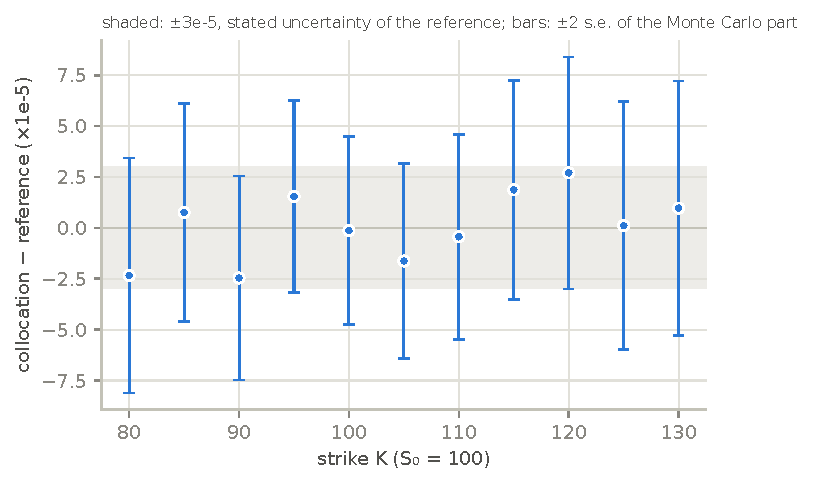
\includegraphics[width=0.78\textwidth]{figs/fig_strikes.pdf}
\caption{Collocation price minus reference price for eleven strikes (base parameters), in units of
$10^{-5}$. Bars show two standard errors of the Monte Carlo part of the reference; the shaded band is the
uncertainty $\pm3\times10^{-5}$ quoted for it.}
\label{fig:strikes}
\end{figure}

\subsection{Convergence in time and space}\label{sec:convergence}

\paragraph{Time.} We fix the spatial grid ($N_x=273$, $N_v=61$) and double the number of time steps from
800 to \num{25600}. Table~\ref{tab:time} shows the at-the-money price. Successive differences shrink by a
factor of $3.98$ to $4.00$, so the error is of second order. After one Richardson step the differences
shrink by a factor close to eight, which is the cubic term produced by the Rannacher steps. With two
levels of extrapolation over $N_t=1600,3200,6400$ the remaining time error, measured against the same
extrapolation over $6400,\dots,25600$, is below $5\times10^{-10}$ for the payoff and $5\times10^{-11}$ for a
smoothed terminal condition. For comparison, the time error of plain Crank--Nicolson with 1600 steps is
$1.5\times10^{-4}$ here, larger than the spatial error on this grid; the time step, not the grid, is what
limits a naive computation.

\begin{table}[t]
\centering
\caption{Time convergence of the at-the-money price ($K=100$, $N_x=273$, $N_v=61$). $d$: difference to
the previous row; $R_1$: one Richardson step \eqref{eq:richardson}; $d_{R}$: difference of $R_1$ to the
previous row.}
\label{tab:time}
\small
\begin{tabular}{rcccccc}
\toprule
$N_t$ & price & $d$ & ratio & $R_1$ & $d_R$ & ratio\\
\midrule
800   & 7.0331102118 & & & & &\\
1600  & 7.0326707632 & $-4.39\times10^{-4}$ & & 7.0325242803 & &\\
3200  & 7.0325604209 & $-1.10\times10^{-4}$ & 3.98 & 7.0325236401 & $-6.4\times10^{-7}$ &\\
6400  & 7.0325327736 & $-2.76\times10^{-5}$ & 3.99 & 7.0325235579 & $-8.2\times10^{-8}$ & 7.78\\
12800 & 7.0325258540 & $-6.92\times10^{-6}$ & 4.00 & 7.0325235474 & $-1.0\times10^{-8}$ & 7.89\\
25600 & 7.0325241231 & $-1.73\times10^{-6}$ & 4.00 & 7.0325235461 & $-1.3\times10^{-9}$ & 7.94\\
\bottomrule
\end{tabular}
\end{table}

\paragraph{Space.} With the time error removed in this way we refine the $x$-grid over ten levels,
$k=4,6,8,11,16,23,32,47,64,94$, which is $N_x$ from 69 to 1599 with the fixed map of
Section~\ref{sec:method}, and keep $N_v=61$. We estimate the order from three consecutive levels without a
reference solution: if $P(k)=P_\infty + Ck^{-q}$, the ratio of successive differences determines $q$. The
$v$-error does not affect these differences: repeating two levels with $N_v=91$ changes the differences by at
most $3\times10^{-10}$, while the differences themselves are $10^{-8}$ to $10^{-6}$.

To separate the effect of the kink we run two terminal conditions: the payoff \eqref{eq:terminal}, and the
smooth function $\frac12(\sqrt{x^2+\varepsilon^2}-x)$ with $\varepsilon=0.25$. Figure~\ref{fig:order} shows
the differences for $K=100$, and Table~\ref{tab:order} lists the last order estimates.

\begin{figure}[t]
\centering
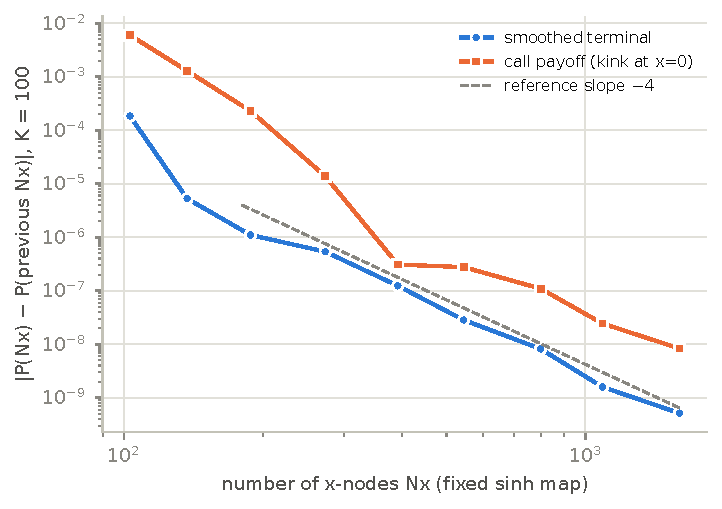
\includegraphics[width=0.78\textwidth]{figs/fig_order.pdf}
\caption{Spatial convergence at $K=100$: absolute difference between prices on consecutive $x$-grids,
plotted at the finer grid. Time error removed by two-level Richardson extrapolation; $N_v=61$.}
\label{fig:order}
\end{figure}

\begin{table}[t]
\centering
\caption{Spatial order estimated from three consecutive grids, for the last four triples (finest on the
right). Payoff estimates are shown only after the differences stop changing sign.}
\label{tab:order}
\small
\begin{tabular}{llcccc}
\toprule
terminal condition & $K$ & & & & finest\\
\midrule
smoothed & 90  & 3.80 & 3.90 & 3.96 & 3.96\\
smoothed & 100 & 3.94 & 3.97 & 3.99 & 3.99\\
smoothed & 110 & 2.11 & 3.43 & 3.72 & 3.92\\
payoff   & 90  & 3.60 & 3.80 & 3.91 & 3.96\\
payoff   & 100 & & 3.06 & 3.61 & 3.83\\
payoff   & 110 & & 2.79 & 3.56 & 3.82\\
\bottomrule
\end{tabular}
\end{table}

With the smooth terminal condition the estimates rise to $3.96$ and $3.99$ for $K=90$ and $100$ and still
move up for $K=110$. The observed order thus approaches four from below. This is what one should expect.
For maximally smooth splines of odd degree $p$, collocation at Greville points is known to converge more
slowly than Galerkin approximation in the same space \citep{Auricchio2010,Anitescu2015}. On a smooth
two-point boundary value problem, $-u''+u=f$ with $u=\sin\pi x$, our implementation converges in the
maximum norm at the rate $p-1$: $4.00$ for quintics and $2.00$ for cubics. We do not claim an
established order: the estimates are still increasing, and in our experience a rising slope is the
typical signature of a pre-asymptotic range.

With the actual payoff the behaviour is different at first. Between $N_x=69$ and $273$ the error falls from
$5$--$9\times10^{-3}$ to below $10^{-6}$, much faster than any fixed rate, and then the differences change
sign. After that the estimates climb towards four as well, reaching $3.82$ to $3.96$ on the finest grids.
At these resolutions the kink does not reduce the rate below that of the smooth problem. We have not
analysed why; a plausible reason is that the kink sits on the line $x=0$ while the price is read at
$x_0\approx1$, so that the local error of the payoff interpolation near $x=0$ is not the dominant term at
the readout point. On the geometric twin, where the kink coincides with the readout point, the picture is
different (Section~\ref{sec:geo}).

For practical purposes the relevant number is the size of the spatial error rather than its order. At
$N_x=273$ the difference to the finest grid is at most $7.3\times10^{-7}$ over the three strikes, forty times
smaller than the uncertainty of the reference.

\subsection{Parameter regimes and domain truncation}\label{sec:regimes}

We now leave the base parameters and vary one parameter at a time: $\rho\in\{-0.9,-0.7,0,0.5,0.9\}$,
$\xi\in\{0.3,0.6,1.5\}$ (Feller ratio $2\kappa\theta/\xi^2$ from $2.0$ down to $0.08$) and
$T\in\{0.25,0.5,3,5\}$. For each regime we compute a reference as in Section~\ref{sec:e8} (four million
paths and 256 steps for $T\le1$, with runs at 64 and 1024 steps added for $\rho=0.9$; 1024 and 2048 steps
pooled for $T\ge3$; the base set uses the reference of Table~\ref{tab:ref}) and a collocation price with
$N_x=392$, $N_v=61$ and time extrapolation.

The first pass through the regimes did not agree everywhere, and the disagreements are instructive. At
$\xi=1.5$ the collocation prices were above the reference by $6\times10^{-4}$ and $5\times10^{-4}$ for
$K=90$ and $100$, eight standard errors. We checked the reference first: the bound was unchanged to eight
digits under changes of damping and quadrature, and the Monte Carlo part showed no trend between 64, 256 and
1024 steps. On the solver side, refining $N_x$ or $N_v$ or changing the clustering changed the price by at
most $5\times10^{-6}$. Moving the variance cut-off from $v_{\max}=1.5$ to $3$ changed it by
$-7.2\times10^{-4}$, and moving it further to $5$ changed it by at most $5\times10^{-6}$. The cut-off was
the whole discrepancy. At the base value $\xi=1$ the same change of cut-off moves the price by less than
$10^{-5}$, which is why the default was adequate there. At $T=5$ we found the same kind of error at the
other end of the domain: moving $x_{\max}$ from 8 to 12 changed the price by $+2.7$ to $+4.4\times10^{-4}$,
while moving $x_{\min}$ or $v_{\max}$ changed it by less than $3\times10^{-5}$. Table~\ref{tab:trunc}
collects these tests.

\begin{table}[t]
\centering
\caption{Sensitivity of collocation prices to one change at a time, for the two regimes where the first
comparison failed and for $T=3$. Changes are new minus old price.}
\label{tab:trunc}
\small
\begin{tabular}{llccc}
\toprule
regime & change & $K=90$ & $K=100$ & $K=110$\\
\midrule
$\xi=1.5$ & $v_{\max}$: $1.5\to3$ & $-7.2\times10^{-4}$ & $-4.3\times10^{-4}$ & $-9.1\times10^{-5}$\\
          & $v_{\max}$: $3\to5$   & $-5.0\times10^{-6}$ & $-1.1\times10^{-6}$ & $+2.9\times10^{-6}$\\
          & $N_x$: $392\to545$     & $+1\times10^{-7}$   & $+7\times10^{-7}$   & $+4.8\times10^{-6}$\\
          & $N_v$: $61\to91$; clustering $\alpha_v$: $0.15\to0.05$ & $<10^{-7}$ & $<10^{-7}$ & $<10^{-7}$\\
$T=5$     & $x_{\max}$: $8\to12$  & $+2.7\times10^{-4}$ & $+3.5\times10^{-4}$ & $+4.4\times10^{-4}$\\
          & $x_{\min}$: $-2\to-3$ & $+2.6\times10^{-5}$ & $+1.3\times10^{-5}$ & $+7.3\times10^{-6}$\\
          & $x\in[-3,12]\to[-4,16]$ & $+3.9\times10^{-5}$ & $+6.1\times10^{-5}$ & $+8.0\times10^{-5}$\\
          & $v_{\max}$: $3\to5\to8$ & $<2\times10^{-5}$ & $<2\times10^{-5}$ & $<2\times10^{-5}$\\
$T=3$     & $v_{\max}$: $3\to5\to8$ & $<4\times10^{-6}$ & $<4\times10^{-6}$ & $<4\times10^{-6}$\\
          & $x\in[-2,8]\to[-3,12]$ & $+2.7\times10^{-5}$ & $+3.7\times10^{-5}$ & $+4.9\times10^{-5}$\\
\bottomrule
\end{tabular}
\end{table}

Neither error can be found by refining the grid, because refinement does not move the boundary: the
solutions converged smoothly, just to a slightly wrong limit. Both were found only because an independent
reference was available at the $10^{-5}$ level. We draw a practical conclusion: in the Heston setting the
truncation of the domain has to be checked separately for each parameter regime, by moving the boundary,
and the default that works at one parameter set does not transfer. Heavier vol-of-vol spreads the
variance distribution, and longer maturities spread the similarity variable.

After widening the domain where needed ($v_{\max}=3$ for all regimes with $T\le1$; $x\in[-3,12]$ at $T=3$;
$x\in[-4,16]$ with $N_x=545$ at $T=5$), the comparison is shown in Figure~\ref{fig:regimes}, with the
numbers in Table~\ref{tab:regimes}. Of the 39 standardised differences, 38 lie within two standard errors,
and their sum of squares is $\chi^2=45.6$ for 39 degrees of freedom. The one exception is $\rho=0.9$,
$K=90$, at $+2.9$ standard errors. There the grid matters: going from $N_x=392$ to $545$ moved this price by
$-4.6\times10^{-5}$, the largest refinement effect we saw, and the value shown is already the finer one.
With strong positive correlation the mixed term $-\rho\xi vx\,w_{xv}$ is large and the solution needs finer
$x$-resolution. The standard errors of the references range from $6\times10^{-6}$ at $T=0.25$ to
$1.9\times10^{-4}$ at $T=5$.

\begin{figure}[t]
\centering
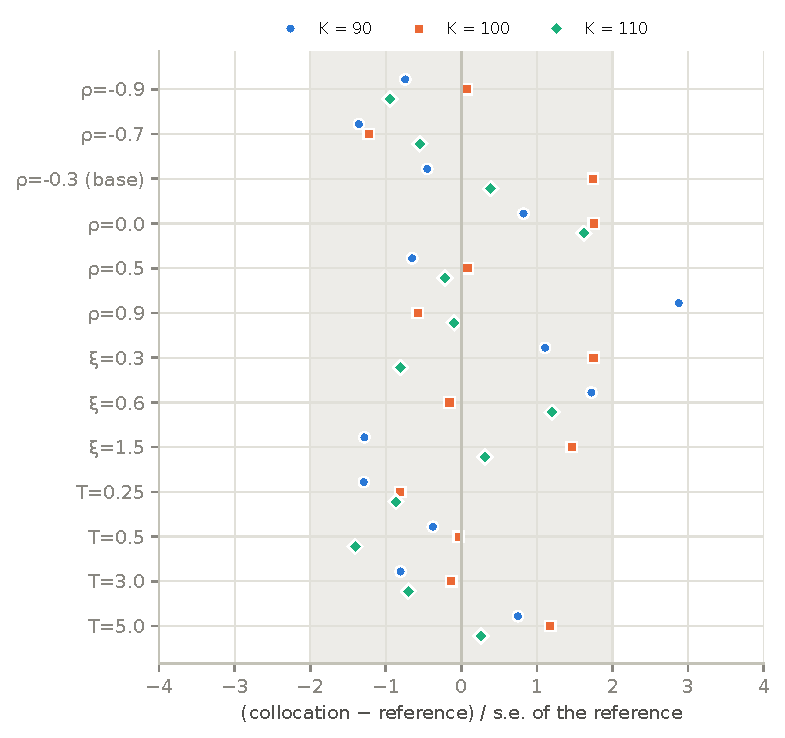
\includegraphics[width=0.72\textwidth]{figs/fig_regimes.pdf}
\caption{Collocation minus reference, divided by the standard error of the reference, for thirteen
parameter regimes and three strikes. One parameter is changed at a time from the base set ($\rho=-0.3$,
$\xi=1$, $T=1$). The shaded band is $\pm2$.}
\label{fig:regimes}
\end{figure}

\subsection{Comparison with ADI}\label{sec:adi}

To compare with a standard method we implemented the modified Craig--Sneyd ADI scheme of
\citet{inthoutFoulon2010} for the same equation \eqref{eq:pde}, on the same domain and with the same
boundary conditions: second-order central differences on stretched grids clustered at $x=0$ and $v=0$,
a second-order one-sided difference in $v$ on the degenerate boundary, $\theta=1/3$, four Rannacher steps,
and bicubic interpolation for the readout. Because the coefficients do not depend on time, all
factorisations of the ADI stages are also computed once, outside the time loop. Without this the
comparison would be unfair to ADI.

Figure~\ref{fig:comparator} plots the largest error over the three strikes against the time for one solve
(each solve prices all three strikes, for both methods). The error is measured against the converged
collocation price, which agrees with the reference within its uncertainty
(Section~\ref{sec:arith}); using the reference itself would cut off the collocation curves at
$3\times10^{-5}$. Plain Crank--Nicolson collocation reaches an error of $10^{-3}$ in about two seconds and
$10^{-4}$ in about eight. With two levels of extrapolation in time it reaches $2\times10^{-5}$ in 14 seconds
and $7\times10^{-7}$ in 76 seconds. ADI needs 25 seconds for $5\times10^{-3}$ on a $961\times121$ grid, and its
error falls roughly like $t^{-1.3}$ with the computing time $t$. At an equal cost of about three seconds
the collocation error is about 150 times smaller. On the finer ADI grids the error at $K=110$ is $1.4$ to $1.8$
times the error at the money, so a comparison at $K=100$ alone understates the difference. The individual runs are
listed in Table~\ref{tab:comp}.

\begin{figure}[t]
\centering
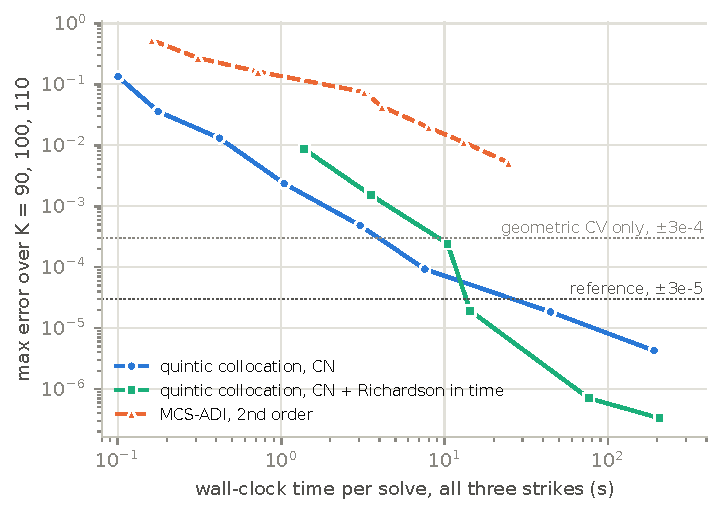
\includegraphics[width=0.8\textwidth]{figs/fig_comparator.pdf}
\caption{Largest error over $K=90,100,110$ against wall-clock time for one solve, arithmetic problem, base
parameters. Errors are relative to the converged collocation price. Horizontal lines mark the uncertainty
of the reference of Table~\ref{tab:ref} and of a Monte Carlo estimate with the geometric control
variate only.}
\label{fig:comparator}
\end{figure}

On the geometric twin the comparison is less one-sided. Its coefficients depend on time, so collocation
has to factorise its system at every step, while ADI only solves banded one-dimensional systems. At the
money, with $N_t=800$, collocation reaches errors of $1.6\times10^{-3}$, $7.3\times10^{-4}$,
$4.1\times10^{-4}$ and $1.8\times10^{-4}$ in 7, 11, 25 and 43 seconds. ADI, with the better of two
clusterings at $v=0$, reaches $1.9\times10^{-2}$, $4.3\times10^{-3}$, $1.8\times10^{-3}$ and
$9.9\times10^{-4}$ in 8, 16, 26 and 36 seconds. Collocation is still ahead at comparable cost, by a factor
of four to twelve, but far less than on the arithmetic problem, where the time-independent operator lets it
factorise once.

The two methods also respond in opposite ways to the clustering of the grid at $v=0$. On the geometric
twin with $N_t=1600$, reducing the clustering width $\alpha_v$ from $0.4$ to $0.005$ lowers the ADI error
at the money from $7.3\times10^{-3}$ to $3.9\times10^{-3}$ ($161\times61$ grid) but raises the collocation
error from $2.4\times10^{-4}$ to $4.3\times10^{-4}$ ($41\times21$ grid). The second-order finite
difference scheme benefits from resolution near the degenerate boundary; the quintic basis does not need it.
How sensitive a solver is to this choice is therefore a property of the method, not only of the problem,
which is worth keeping in mind when results for different Heston schemes are compared.

\subsection{Comparison with published values}\label{sec:published}

\citet{FusaiKyriakou2016} report, in their Table~9, maximal lower bounds for three Heston parameter sets
taken from \citet{EwaldMenkensTing2013}, together with the ADI and Monte Carlo prices of that paper. All
three sets satisfy the Feller condition. Table~\ref{tab:published} puts these numbers next to ours.

\begin{table}[t]
\centering
\caption{Published values for the Heston sets of \citet[Table~1]{EwaldMenkensTing2013}
($S_0=K=100$, $T=1$, $q=0$; set 1: $\kappa=4.75$, $\theta=v_0=0.0483$, $\xi=0.55$, $\rho=-0.569$, $r=0.04$;
set 2: $\kappa=3$, $\theta=v_0=0.1$, $\xi=0.2$, $\rho=0.7$, $r=0.1$; set 3: $\kappa=7$, $\theta=0.05$,
$v_0=0.075$, $\xi=0.3$, $\rho=-0.4$, $r=0.07$) and our results. EMT MC: range of their Monte Carlo
estimates over schemes. Our MC: quadratic-exponential scheme with geometric control variate (2M paths)
and full-truncation Euler without any control variate (16M paths, pooled over 100 to 800 time steps).}
\label{tab:published}
\small
\begin{tabular}{lccc}
\toprule
& set 1 & set 2 & set 3\\
\midrule
\citet{FusaiKyriakou2016}, MLB & 5.854 & 9.323 & 7.123\\
\citet{EwaldMenkensTing2013}, ADI & 5.852839 & 9.323261 & 7.122597\\
\citet{EwaldMenkensTing2013}, MC & 5.851--5.871 & 9.321--9.334 & 7.123--7.136\\
\midrule
MLB, this paper & 5.86532 & 9.32373 & 7.12900\\
MC estimate of the same bound & $5.86510\pm0.00014$ & $9.32409\pm0.00053$ & $7.12889\pm0.00019$\\
MC price, QE with control variate & $5.86576\pm0.00014$ & $9.32549\pm0.00053$ & $7.12949\pm0.00019$\\
MC price, Euler, no control variate & $5.8665\pm0.0019$ & $9.3257\pm0.0035$ & $7.1311\pm0.0024$\\
Collocation & 5.86599 & 9.32513 & 7.12960\\
\bottomrule
\end{tabular}
\end{table}

We could not reproduce the three MLB values. Our bound is higher by $0.0113$, $0.0007$ and $0.0060$, or
$0.19\%$, $0.01\%$ and $0.08\%$ of the price. In practical terms the numbers are close, but on set 1 the
gap is about eighty standard errors of our simulation of the same quantity, so it is not noise. Several
causes can be excluded. Our implementation reproduces Table~10 of the same paper to all printed digits
(Table~\ref{tab:fk10}), is stable under changes of its numerical parameters, and agrees with a direct
simulation of the bound. The optimisation over $\lambda$ cannot explain the gap either, because the bound
is flat near its maximum: even $\lambda=\ln K$, without any optimisation, gives $5.8645$ on set 1. Seven
alternative readings of the parameters (the sign of $\rho$, $\xi$ against $\xi^2$ or $\sqrt\xi$, variance
against volatility for $v_0$ and $\theta$, and the limits $\rho=0$ and $\xi=0$) do not reproduce the table.
Taken over all three sets the reading we use is the closest, although $\rho=0$ comes nearer on set~1 and
$\xi=0$ on set~3. Finally, we simulated the bound itself at our $\lambda^\ast$ with the full-truncation Euler scheme of
\citet{LordKoekkoekvanDijk2010} and no control variate, which shares nothing with our other computations
except the model and the value of $\lambda^\ast$. For set 1 this gives $\LB(\lambda^\ast)=5.8658\pm0.0019$,
six standard errors above the published value. Since any $\LB(\lambda)$ is a lower bound for the maximum,
the published value is not consistent with the model as printed. Two causes we cannot check: how the transform for the continuous average under
Heston was evaluated, since the paper describes this step only in outline, and whether the table was
computed for a specification other than the one printed.

Two observations may help a reader who wants to pursue this. The published bounds agree to three digits
with the ADI prices of \citet{EwaldMenkensTing2013}, which were computed on a uniform grid of 1000 points in
each of $x$, $v$ and $t$, with a Dirichlet condition at $v_{\max}=3$. And the Monte Carlo estimates that
paper reports for set 1 range from $5.851$ to $5.871$ depending on the scheme, a spread wider than the gap
we are discussing. Our collocation price and our two simulations with different schemes agree with each
other within two standard errors of the simulations, and within $6\times10^{-6}$ when the bound is used
as a control variate in the Euler simulation. For the same reason the published values are of limited use
as an external check of a solver. Our collocation prices lie above the published bounds, as they must, but
by a margin that mostly reflects the discrepancy discussed here.
